\documentclass[a4paper,11pt]{article}
\usepackage[utf8]{inputenc}
\usepackage[T1]{fontenc}
\usepackage{amsmath,amssymb}
\usepackage[a4paper,left=2cm,right=2cm,top=3.6cm,bottom=2.3cm,headheight=1.1cm,headsep=0.6cm,footskip=1cm]{geometry}
\usepackage{xcolor}
\usepackage{tikz}
\usetikzlibrary{calc,arrows.meta}
\usepackage{fancyhdr}
\usepackage{lastpage}
\usepackage{tabularx}
\usepackage{array}
\usepackage[most]{tcolorbox}
\usepackage{enumitem}
\usepackage{needspace}

\definecolor{navy}{HTML}{1F3A5F}
\definecolor{teal}{HTML}{0F8B7D}
\definecolor{amber}{HTML}{D9822B}
\definecolor{softbg}{HTML}{F4F7FA}
\definecolor{brick}{HTML}{B03A2E}
\definecolor{violetx}{HTML}{6C4AB6}
\newcommand{\dis}{\displaystyle}
\newcommand{\Me}{\mathrm{Me}}
\newcommand{\Mo}{\mathrm{Mo}}

\setlength{\parindent}{0pt}
\renewcommand{\arraystretch}{1.35}

% ---------- header berwarna navy ----------
\pagestyle{fancy}
\fancyhf{}
\renewcommand{\headrulewidth}{0pt}
\fancyhead[L]{%
  \begin{tikzpicture}[remember picture,overlay]
    \fill[navy] ([yshift=-1.2cm]current page.north west) rectangle ([yshift=-3.15cm]current page.north east);
    \fill[teal] ([yshift=-3.15cm]current page.north west) rectangle ([yshift=-3.25cm]current page.north east);
  \end{tikzpicture}%
  \color{white}\bfseries\large Latihan Soal Statistika}
\fancyhead[R]{\color{white}\small Diunduh dari website \textbf{Math1729}\ \,|\,\ 4 Oktober 2026}
\fancyfoot[L]{\small\color{navy}Math1729 --- Statistika}
\fancyfoot[R]{\small\color{navy}Halaman \thepage\ dari \pageref{LastPage}}

% ---------- komponen ----------
\newcounter{no}
\newcommand{\bagian}[2]{\par\Needspace{6\baselineskip}\vspace{1.0em}\noindent
  \begin{tcolorbox}[colback=navy,colframe=navy,coltext=white,boxrule=0pt,arc=2pt,left=6pt,right=6pt,top=3pt,bottom=3pt]
  \textbf{#1}\hfill{\small #2}\end{tcolorbox}\setcounter{no}{0}\par\vspace{-0.3em}}
\newcommand{\tingkat}[2]{\par\Needspace{7\baselineskip}\vspace{0.6em}\noindent
  {\color{teal}\rule{3pt}{1.1em}}\ {\color{navy}\bfseries #1}\ {\small\color{gray}--- #2}\par\vspace{0.1em}}
\newcommand{\soal}[2]{\par\vspace{0.75em}\stepcounter{no}\noindent
  \begin{minipage}[t]{1.8em}\textbf{\theno.}\end{minipage}%
  \begin{minipage}[t]{\dimexpr\linewidth-1.8em\relax}#1\par\vspace{0.35em}#2\end{minipage}\par}
\newcommand{\poin}[1]{\hfill{\small\color{navy}[#1 poin]}}

% teks di kiri, gambar di kanan
\newcommand{\gbr}[2]{\noindent\begin{minipage}[t]{0.58\linewidth}#1\end{minipage}\hfill\raisebox{\ht\strutbox}{\begin{minipage}[t]{0.39\linewidth}\vspace{0pt}\centering#2\end{minipage}}}

\begin{document}
\thispagestyle{fancy}

\begin{center}
  {\color{navy}\fontsize{22}{26}\selectfont\bfseries Latihan Soal Statistika\par}
  \vspace{2pt}
  {\color{teal}\large Mean, Median, dan Modus (Data Tunggal dan Berkelompok)\par}
\end{center}
\vspace{2pt}
\begin{tcolorbox}[colback=softbg,colframe=navy!40,boxrule=0.6pt,arc=3pt,left=8pt,right=8pt,top=5pt,bottom=5pt]
\noindent\textbf{Nama} : \rule{4.6cm}{0.4pt}\hfill\textbf{Kelas} : \rule{2.2cm}{0.4pt}\hfill\textbf{Skor} : \rule{2.2cm}{0.4pt}
\end{tcolorbox}
\vspace{2pt}
\begin{tcolorbox}[colback=white,colframe=teal,boxrule=0.8pt,arc=3pt,left=8pt,right=8pt,top=4pt,bottom=4pt,title={\bfseries Petunjuk Pengerjaan},coltitle=white,fonttitle=\small]
\small
\begin{enumerate}[leftmargin=1.4em,itemsep=1pt,topsep=1pt]
\item Soal terdiri atas \textbf{20 pilihan ganda} (5 mudah, 5 sedang, 5 sulit, 5 HOTS), \textbf{5 isian singkat}, dan \textbf{5 uraian (essay)}. Soal disusun berjenjang dari mudah sampai HOTS dan sebagian bergaya UTBK. Alokasi waktu yang disarankan: 120 menit.
\item Skor: pilihan ganda 2 poin, isian singkat 4 poin, uraian 8 poin per soal (total 100 poin). Tidak ada pengurangan skor untuk jawaban salah.
\item Notasi: $\bar{x}$ rata-rata (mean), $\Me$ median, $\Mo$ modus, $n$ banyak data, $f$ frekuensi, $t_b$ tepi bawah kelas, $p$ panjang kelas. Pada data berkelompok, kelas bernilai bulat memiliki tepi bawah $=$ batas bawah $-0{,}5$. Gambar tidak selalu digambar sesuai skala.
\item Bilangan desimal ditulis dengan tanda koma. Jika perlu, bulatkan hasil sampai dua angka desimal.
\item Kalkulator tidak diperkenankan.
\end{enumerate}
\end{tcolorbox}

% =====================================================================
\bagian{A. Pilihan Ganda}{20 soal $\times$ 2 poin = 40 poin. Pilih satu jawaban yang paling tepat.}

\tingkat{Tingkat Mudah}{soal 1 sampai 5}
\soal{Banyak buku yang dibaca delapan siswa selama liburan adalah $4,6,5,8,7,6,9,5$. Rata-rata banyak buku yang dibaca adalah \dots.}{\begin{tabularx}{\linewidth}{@{}*{5}{X}@{}}\textbf{A.}\;$6$ & \textbf{B.}\;$6{,}25$ & \textbf{C.}\;$6{,}5$ & \textbf{D.}\;$6{,}75$ & \textbf{E.}\;$7$\end{tabularx}}
\soal{Banyak pengunjung sebuah perpustakaan selama delapan hari berturut-turut adalah $14,9,21,11,17,12,8,16$ orang. Median data tersebut adalah \dots.}{\begin{tabularx}{\linewidth}{@{}*{5}{X}@{}}\textbf{A.}\;$12$ & \textbf{B.}\;$12{,}5$ & \textbf{C.}\;$13$ & \textbf{D.}\;$13{,}5$ & \textbf{E.}\;$14$\end{tabularx}}
\soal{\gbr{Diagram batang pada gambar menunjukkan nilai ulangan matematika $20$ siswa. Rata-rata nilai ulangan tersebut adalah \dots.}{%
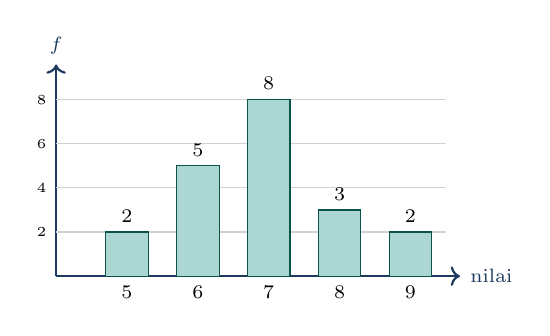
\begin{tikzpicture}[x=0.9cm,y=0.28cm]
\draw[->,thick,navy] (0,0)--(5.7,0) node[right,font=\scriptsize]{nilai};
\draw[->,thick,navy] (0,0)--(0,9.6) node[above,font=\scriptsize]{$f$};
\foreach \y in {2,4,6,8}{\draw[gray!35] (0,\y)--(5.5,\y); \node[left,font=\tiny] at (0,\y) {\y};}
\foreach \i/\vv/\fr in {1/5/2,2/6/5,3/7/8,4/8/3,5/9/2}{
  \fill[teal!35,draw=teal!60!black] (\i-0.3,0) rectangle (\i+0.3,\fr);
  \node[font=\scriptsize,above] at (\i,\fr) {\fr};
  \node[font=\scriptsize,below] at (\i,0) {\vv};}
\end{tikzpicture}}}{\begin{tabularx}{\linewidth}{@{}*{5}{X}@{}}\textbf{A.}\;$6{,}6$ & \textbf{B.}\;$6{,}7$ & \textbf{C.}\;$6{,}8$ & \textbf{D.}\;$6{,}9$ & \textbf{E.}\;$7{,}0$\end{tabularx}}
\soal{\gbr{Diagram lingkaran pada gambar menunjukkan ekstrakurikuler pilihan $240$ siswa. Banyak siswa yang memilih ekstrakurikuler yang paling diminati (modus) adalah \dots.}{%
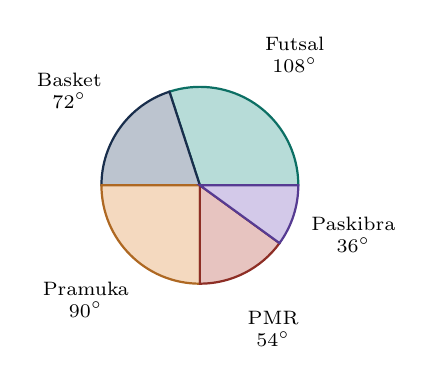
\begin{tikzpicture}
\def\R{1.25}
\foreach \sa/\ea/\cl/\nm/\dg in {0/108/teal/Futsal/108,108/180/navy/Basket/72,180/270/amber/Pramuka/90,270/324/brick/PMR/54,324/360/violetx/Paskibra/36}{
  \fill[\cl!30,draw=\cl!80!black,thick] (0,0)--(\sa:\R) arc (\sa:\ea:\R)--cycle;
  \pgfmathsetmacro{\ma}{(\sa+\ea)/2}
  \node[font=\scriptsize,align=center] at (\ma:{\R+0.8}) {\nm\\$\dg^\circ$};}
\end{tikzpicture}}}{\begin{tabularx}{\linewidth}{@{}*{5}{X}@{}}\textbf{A.}\;$72$ & \textbf{B.}\;$80$ & \textbf{C.}\;$90$ & \textbf{D.}\;$108$ & \textbf{E.}\;$120$\end{tabularx}}
\soal{Rata-rata nilai ulangan $5$ siswa adalah $78$. Setelah seorang siswa susulan mengikuti ulangan, rata-rata nilai keenam siswa menjadi $80$. Nilai siswa susulan tersebut adalah \dots.}{\begin{tabularx}{\linewidth}{@{}*{5}{X}@{}}\textbf{A.}\;$82$ & \textbf{B.}\;$84$ & \textbf{C.}\;$86$ & \textbf{D.}\;$88$ & \textbf{E.}\;$90$\end{tabularx}}

\tingkat{Tingkat Sedang}{soal 6 sampai 10}
\soal{Suatu data berkelompok yang sebarannya tidak terlalu condong memiliki rata-rata $58$ dan median $56$. Dengan hampiran $\Mo\approx3\,\Me-2\,\bar{x}$, modus data tersebut kira-kira \dots.}{\begin{tabularx}{\linewidth}{@{}*{5}{X}@{}}\textbf{A.}\;$46$ & \textbf{B.}\;$48$ & \textbf{C.}\;$50$ & \textbf{D.}\;$52$ & \textbf{E.}\;$54$\end{tabularx}}
\soal{Nilai ujian sejumlah siswa memiliki rata-rata $56$, median $52$, dan modus $48$. Setiap nilai $x$ diubah menjadi $y=1{,}5x+4$. Selisih rata-rata dan modus nilai yang baru adalah \dots.}{\begin{tabularx}{\linewidth}{@{}*{5}{X}@{}}\textbf{A.}\;$8$ & \textbf{B.}\;$10$ & \textbf{C.}\;$12$ & \textbf{D.}\;$14$ & \textbf{E.}\;$16$\end{tabularx}}
\soal{\gbr{Histogram pada gambar menunjukkan waktu tempuh (menit) $40$ siswa dari rumah ke sekolah. Modus data tersebut adalah \dots.}{%
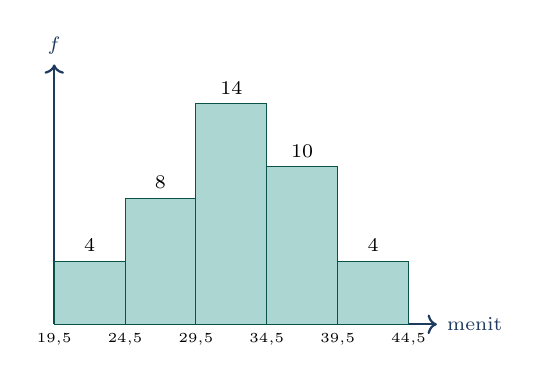
\begin{tikzpicture}[x=0.9cm,y=0.2cm]
\draw[->,thick,navy] (0,0)--(5.4,0) node[right,font=\scriptsize]{menit};
\draw[->,thick,navy] (0,0)--(0,16.5) node[above,font=\scriptsize]{$f$};
\foreach \i/\hh in {1/4,2/8,3/14,4/10,5/4}{
  \fill[teal!35,draw=teal!60!black] (\i-1,0) rectangle (\i,\hh);
  \node[font=\scriptsize,above] at (\i-0.5,\hh) {\hh};}
\foreach \i/\lab in {0/19{,}5,1/24{,}5,2/29{,}5,3/34{,}5,4/39{,}5,5/44{,}5}{\node[font=\tiny,below] at (\i,0) {$\lab$};}
\end{tikzpicture}}}{\begin{tabularx}{\linewidth}{@{}*{5}{X}@{}}\textbf{A.}\;$32$ & \textbf{B.}\;$32{,}5$ & \textbf{C.}\;$33$ & \textbf{D.}\;$33{,}5$ & \textbf{E.}\;$34$\end{tabularx}}
\soal{\gbr{Tabel di samping menyajikan berat badan $40$ siswa. Median berat badan tersebut adalah \dots.}{%
\small
\begin{tabular}{@{}c|c@{}}
\hline
\textbf{Berat (kg)} & \textbf{Frekuensi}\\ \hline
$45$--$49$ & $6$\\
$50$--$54$ & $9$\\
$55$--$59$ & $10$\\
$60$--$64$ & $8$\\
$65$--$69$ & $7$\\ \hline
\end{tabular}}}{\begin{tabularx}{\linewidth}{@{}*{5}{X}@{}}\textbf{A.}\;$55$ & \textbf{B.}\;$55{,}5$ & \textbf{C.}\;$56$ & \textbf{D.}\;$56{,}5$ & \textbf{E.}\;$57$\end{tabularx}}
\soal{Tinggi tanaman kacang diukur dengan ketelitian $0{,}1$ cm dan disajikan dalam tabel distribusi frekuensi. Salah satu kelasnya adalah $14{,}5$--$16{,}4$. Tepi bawah dan panjang kelas tersebut berturut-turut adalah \dots.}{\begin{tabularx}{\linewidth}{@{}*{3}{X}@{}}\textbf{A.}\;$14{,}45$ dan $2{,}0$ & \textbf{B.}\;$14{,}45$ dan $1{,}9$ & \textbf{C.}\;$14{,}5$ dan $1{,}9$\\[3pt] \textbf{D.}\;$14{,}5$ dan $2{,}0$ & \textbf{E.}\;$14{,}4$ dan $2{,}0$ & \end{tabularx}}

\tingkat{Tingkat Sulit}{soal 11 sampai 15, setara UTBK}
\soal{Rata-rata nilai $30$ siswa dicatat $65$. Setelah diperiksa, ternyata nilai $84$ tertulis $48$ dan nilai $70$ tertulis $79$. Rata-rata nilai yang sebenarnya adalah \dots.}{\begin{tabularx}{\linewidth}{@{}*{5}{X}@{}}\textbf{A.}\;$65{,}3$ & \textbf{B.}\;$65{,}6$ & \textbf{C.}\;$65{,}9$ & \textbf{D.}\;$66{,}2$ & \textbf{E.}\;$66{,}5$\end{tabularx}}
\soal{\gbr{Ogive ``kurang dari'' pada gambar menyajikan nilai ulangan $50$ siswa. Median data tersebut adalah \dots.}{%
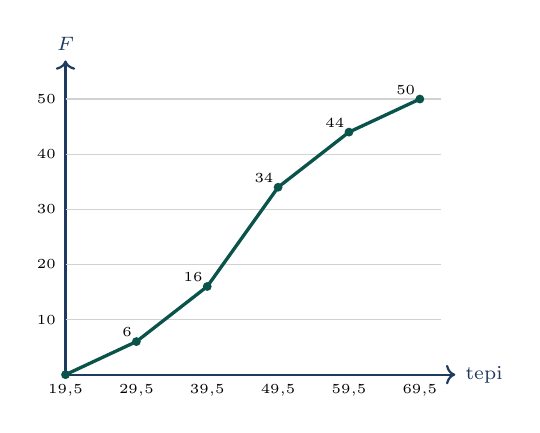
\begin{tikzpicture}[x=0.9cm,y=0.07cm]
\draw[->,thick,navy] (0,0)--(5.5,0) node[right,font=\scriptsize]{tepi};
\draw[->,thick,navy] (0,0)--(0,57) node[above,font=\scriptsize]{$F$};
\foreach \y in {10,20,30,40,50}{\draw[gray!35] (0,\y)--(5.3,\y); \node[left,font=\tiny] at (0,\y) {\y};}
\foreach \i/\lab in {0/19{,}5,1/29{,}5,2/39{,}5,3/49{,}5,4/59{,}5,5/69{,}5}{\node[font=\tiny,below] at (\i,0) {$\lab$};}
\draw[teal!60!black,very thick] (0,0)--(1,6)--(2,16)--(3,34)--(4,44)--(5,50);
\foreach \i/\fk in {0/0,1/6,2/16,3/34,4/44,5/50}{\fill[teal!60!black] (\i,\fk) circle (1.6pt);}
\foreach \i/\fk in {1/6,2/16,3/34,4/44,5/50}{\node[font=\tiny,above left,inner sep=1.5pt] at (\i,\fk) {\fk};}
\end{tikzpicture}}}{\begin{tabularx}{\linewidth}{@{}*{5}{X}@{}}\textbf{A.}\;$43{,}5$ & \textbf{B.}\;$44{,}5$ & \textbf{C.}\;$45$ & \textbf{D.}\;$45{,}5$ & \textbf{E.}\;$46{,}5$\end{tabularx}}
\soal{\gbr{Poligon frekuensi pada gambar menyajikan skor tes sejumlah peserta; sumbu mendatar memuat titik tengah kelas. Rata-rata skor peserta tersebut adalah \dots.}{%
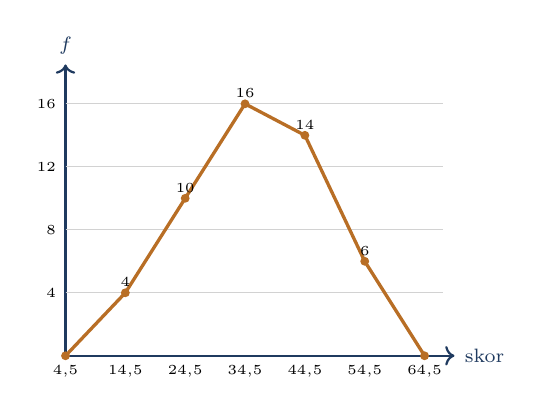
\begin{tikzpicture}[x=0.76cm,y=0.2cm]
\draw[->,thick,navy] (0,0)--(6.5,0) node[right,font=\scriptsize]{skor};
\draw[->,thick,navy] (0,0)--(0,18.5) node[above,font=\scriptsize]{$f$};
\foreach \y in {4,8,12,16}{\draw[gray!35] (0,\y)--(6.3,\y); \node[left,font=\tiny] at (0,\y) {\y};}
\foreach \i/\lab in {0/4{,}5,1/14{,}5,2/24{,}5,3/34{,}5,4/44{,}5,5/54{,}5,6/64{,}5}{\node[font=\tiny,below] at (\i,0) {$\lab$};}
\draw[amber!85!black,very thick] (0,0)--(1,4)--(2,10)--(3,16)--(4,14)--(5,6)--(6,0);
\foreach \i/\fr in {0/0,1/4,2/10,3/16,4/14,5/6,6/0}{\fill[amber!85!black] (\i,\fr) circle (1.6pt);}
\foreach \i/\fr in {1/4,2/10,3/16,4/14,5/6}{\node[font=\tiny,above,inner sep=2pt] at (\i,\fr) {\fr};}
\end{tikzpicture}}}{\begin{tabularx}{\linewidth}{@{}*{5}{X}@{}}\textbf{A.}\;$34{,}5$ & \textbf{B.}\;$35{,}3$ & \textbf{C.}\;$35{,}5$ & \textbf{D.}\;$36{,}1$ & \textbf{E.}\;$36{,}5$\end{tabularx}}
\soal{Perhatikan data $4,5,5,6,6,6,7,8,9,14$ dan pernyataan berikut.
\begin{enumerate}[label=(\arabic*),leftmargin=1.8em,itemsep=0pt,topsep=2pt]
\item Rata-rata data lebih besar daripada median.
\item Jika $14$ diganti $40$, median tidak berubah tetapi rata-rata berubah.
\item Modus data sama dengan median.
\item Jika setiap data dikalikan $2$, selisih rata-rata dan median tetap $1$.
\end{enumerate}
Pernyataan yang benar adalah \dots.}{\begin{tabularx}{\linewidth}{@{}*{3}{X}@{}}\textbf{A.}\;(1), (2), dan (3) saja & \textbf{B.}\;(1) dan (3) saja & \textbf{C.}\;(2) dan (4) saja\\[3pt] \textbf{D.}\;(4) saja & \textbf{E.}\;(1), (2), (3), dan (4) & \end{tabularx}}
\soal{Rata-rata nilai ujian seluruh siswa suatu kelas adalah $72$. Jika rata-rata nilai siswa laki-laki $68$ dan rata-rata nilai siswa perempuan $75$, perbandingan banyak siswa perempuan terhadap banyak siswa laki-laki adalah \dots.}{\begin{tabularx}{\linewidth}{@{}*{5}{X}@{}}\textbf{A.}\;$2:3$ & \textbf{B.}\;$3:4$ & \textbf{C.}\;$1:1$ & \textbf{D.}\;$5:4$ & \textbf{E.}\;$4:3$\end{tabularx}}

\tingkat{Tingkat HOTS}{soal 16 sampai 20, penalaran tingkat tinggi gaya UTBK}
\soal{Lima bilangan bulat positif memiliki rata-rata $8$, median $9$, dan satu-satunya modus $10$. Nilai terkecil yang mungkin dari kelima bilangan tersebut adalah \dots.}{\begin{tabularx}{\linewidth}{@{}*{5}{X}@{}}\textbf{A.}\;$2$ & \textbf{B.}\;$3$ & \textbf{C.}\;$4$ & \textbf{D.}\;$5$ & \textbf{E.}\;$6$\end{tabularx}}
\soal{\gbr{Tabel di samping menyajikan nilai $40$ siswa; frekuensi kelas $30$--$39$ dan $50$--$59$ dinyatakan dengan $p$ dan $q$. Jika median data tersebut adalah $44{,}5$, rata-rata nilai siswa adalah \dots.}{%
\small
\begin{tabular}{@{}c|c@{}}
\hline
\textbf{Nilai} & \textbf{Frekuensi}\\ \hline
$20$--$29$ & $6$\\
$30$--$39$ & $p$\\
$40$--$49$ & $14$\\
$50$--$59$ & $q$\\
$60$--$69$ & $4$\\ \hline
\end{tabular}}}{\begin{tabularx}{\linewidth}{@{}*{5}{X}@{}}\textbf{A.}\;$44$ & \textbf{B.}\;$44{,}5$ & \textbf{C.}\;$45$ & \textbf{D.}\;$45{,}5$ & \textbf{E.}\;$46$\end{tabularx}}
\soal{Lima bilangan $4,6,7,9,x$ memiliki rata-rata yang sama dengan mediannya. Jumlah semua nilai $x$ yang mungkin adalah \dots.}{\begin{tabularx}{\linewidth}{@{}*{5}{X}@{}}\textbf{A.}\;$6{,}5$ & \textbf{B.}\;$10{,}5$ & \textbf{C.}\;$13$ & \textbf{D.}\;$15{,}5$ & \textbf{E.}\;$19{,}5$\end{tabularx}}
\soal{\gbr{Histogram pada gambar menyajikan skor $40$ peserta tes. Hubungan yang benar antara rata-rata $\bar{x}$, median $\Me$, dan modus $\Mo$ data tersebut adalah \dots.}{%
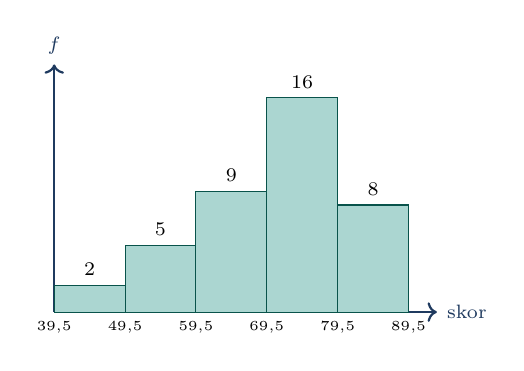
\begin{tikzpicture}[x=0.9cm,y=0.17cm]
\draw[->,thick,navy] (0,0)--(5.4,0) node[right,font=\scriptsize]{skor};
\draw[->,thick,navy] (0,0)--(0,18.5) node[above,font=\scriptsize]{$f$};
\foreach \i/\hh in {1/2,2/5,3/9,4/16,5/8}{
  \fill[teal!35,draw=teal!60!black] (\i-1,0) rectangle (\i,\hh);
  \node[font=\scriptsize,above] at (\i-0.5,\hh) {\hh};}
\foreach \i/\lab in {0/39{,}5,1/49{,}5,2/59{,}5,3/69{,}5,4/79{,}5,5/89{,}5}{\node[font=\tiny,below] at (\i,0) {$\lab$};}
\end{tikzpicture}}}{\begin{tabularx}{\linewidth}{@{}*{3}{X}@{}}\textbf{A.}\;$\Mo<\Me<\bar{x}$ & \textbf{B.}\;$\Me<\Mo<\bar{x}$ & \textbf{C.}\;$\Me<\bar{x}<\Mo$\\[3pt] \textbf{D.}\;$\bar{x}<\Me<\Mo$ & \textbf{E.}\;$\bar{x}=\Me=\Mo$ & \end{tabularx}}
\soal{Dalam suatu kelas terdapat siswa laki-laki dan siswa perempuan. Apakah rata-rata nilai ujian seluruh siswa di kelas itu lebih dari $74$?
\begin{enumerate}[label=(\arabic*),leftmargin=1.8em,itemsep=0pt,topsep=2pt]
\item Rata-rata nilai siswa laki-laki adalah $70$ dan rata-rata nilai siswa perempuan adalah $80$.
\item Banyak siswa perempuan lebih banyak daripada banyak siswa laki-laki.
\end{enumerate}}{\begin{tabularx}{\linewidth}{@{}lX@{}}
\textbf{A.} & Pernyataan (1) SAJA cukup untuk menjawab pertanyaan, tetapi pernyataan (2) SAJA tidak cukup.\\
\textbf{B.} & Pernyataan (2) SAJA cukup untuk menjawab pertanyaan, tetapi pernyataan (1) SAJA tidak cukup.\\
\textbf{C.} & DUA pernyataan BERSAMA-SAMA cukup untuk menjawab pertanyaan, tetapi SATU pernyataan SAJA tidak cukup.\\
\textbf{D.} & Pernyataan (1) SAJA cukup dan pernyataan (2) SAJA cukup untuk menjawab pertanyaan.\\
\textbf{E.} & Pernyataan (1) dan pernyataan (2) tidak cukup untuk menjawab pertanyaan.
\end{tabularx}}

% =====================================================================
\bagian{B. Isian Singkat}{5 soal $\times$ 4 poin = 20 poin. Tuliskan hanya jawaban akhir.}

\tingkat{Tingkat Mudah dan Sedang}{soal 1 dan 2}
\soal{\gbr{Tabel di samping menyajikan nilai ulangan $20$ siswa. Rata-rata nilai ulangan tersebut adalah \dots}{%
\small
\begin{tabular}{@{}c|cccccc@{}}
\hline
Nilai & $5$ & $6$ & $7$ & $8$ & $9$ & $10$\\ \hline
Frekuensi & $2$ & $3$ & $7$ & $5$ & $2$ & $1$\\ \hline
\end{tabular}}}{\hfill Jawaban: \rule{4.5cm}{0.4pt}}
\soal{\gbr{Tabel di samping menyajikan tinggi badan $40$ siswa. Rata-rata tinggi badan siswa tersebut adalah \dots\ cm.}{%
\small
\begin{tabular}{@{}c|c@{}}
\hline
\textbf{Tinggi (cm)} & \textbf{Frekuensi}\\ \hline
$150$--$154$ & $4$\\
$155$--$159$ & $8$\\
$160$--$164$ & $14$\\
$165$--$169$ & $10$\\
$170$--$174$ & $4$\\ \hline
\end{tabular}}}{\hfill Jawaban: \rule{4.5cm}{0.4pt}}

\tingkat{Tingkat Sulit}{soal 3 dan 4}
\soal{\gbr{Ogive ``lebih dari'' pada gambar menyajikan nilai ulangan $40$ siswa. Median data tersebut adalah \dots}{%
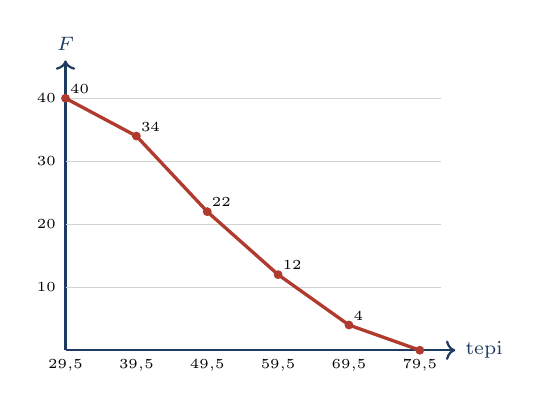
\begin{tikzpicture}[x=0.9cm,y=0.08cm]
\draw[->,thick,navy] (0,0)--(5.5,0) node[right,font=\scriptsize]{tepi};
\draw[->,thick,navy] (0,0)--(0,46) node[above,font=\scriptsize]{$F$};
\foreach \y in {10,20,30,40}{\draw[gray!35] (0,\y)--(5.3,\y); \node[left,font=\tiny] at (0,\y) {\y};}
\foreach \i/\lab in {0/29{,}5,1/39{,}5,2/49{,}5,3/59{,}5,4/69{,}5,5/79{,}5}{\node[font=\tiny,below] at (\i,0) {$\lab$};}
\draw[brick,very thick] (0,40)--(1,34)--(2,22)--(3,12)--(4,4)--(5,0);
\foreach \i/\fk in {0/40,1/34,2/22,3/12,4/4,5/0}{\fill[brick] (\i,\fk) circle (1.6pt);}
\foreach \i/\fk in {0/40,1/34,2/22,3/12,4/4}{\node[font=\tiny,above right,inner sep=1.5pt] at (\i,\fk) {\fk};}
\end{tikzpicture}}}{\hfill Jawaban: \rule{4.5cm}{0.4pt}}
\soal{\gbr{Tabel di samping menyajikan hasil tes sejumlah siswa dengan frekuensi kelas $21$--$30$ dinyatakan dengan $x$. Jika median data tersebut adalah $25$, nilai $x$ adalah \dots}{%
\small
\begin{tabular}{@{}c|c@{}}
\hline
\textbf{Nilai} & \textbf{Frekuensi}\\ \hline
$1$--$10$ & $5$\\
$11$--$20$ & $8$\\
$21$--$30$ & $x$\\
$31$--$40$ & $9$\\
$41$--$50$ & $3$\\ \hline
\end{tabular}}}{\hfill Jawaban: \rule{4.5cm}{0.4pt}}

\tingkat{Tingkat HOTS}{soal 5}
\soal{Rata-rata nilai $40$ siswa adalah $72$. Seperempat siswa dengan nilai terendah memiliki rata-rata $50$, sedangkan seperempat siswa dengan nilai tertinggi memiliki rata-rata $90$. Rata-rata nilai separuh siswa yang berada di tengah adalah \dots}{\hfill Jawaban: \rule{4.5cm}{0.4pt}}

% =====================================================================
\bagian{C. Uraian (Essay)}{5 soal $\times$ 8 poin = 40 poin. Tuliskan langkah penyelesaian dengan lengkap.}

\tingkat{Tingkat Sedang}{soal 1 dan 2}
\soal{Nilai ulangan matematika $20$ siswa adalah sebagai berikut.
\[ \begin{array}{cccccccccc}
7&8&6&9&7&8&5&7&10&8\\
6&7&9&8&7&6&8&7&9&5
\end{array} \]
(a) Susunlah tabel distribusi frekuensi data tersebut.\par
(b) Tentukan rata-rata nilai ulangan.\par
(c) Tentukan median dan modus.\par
(d) Berapa persen siswa yang nilainya lebih dari rata-rata?}{\poin{8}}
\soal{\gbr{Histogram pada gambar menyajikan waktu (menit) yang diperlukan sejumlah peserta untuk menyelesaikan suatu tes.\par\smallskip(a) Tentukan banyak peserta dan persentase peserta yang menyelesaikan tes paling lama $40$ menit.\par(b) Tentukan rata-rata waktu penyelesaian.\par(c) Tentukan median waktu penyelesaian.\par(d) Tentukan modus waktu penyelesaian.}{%
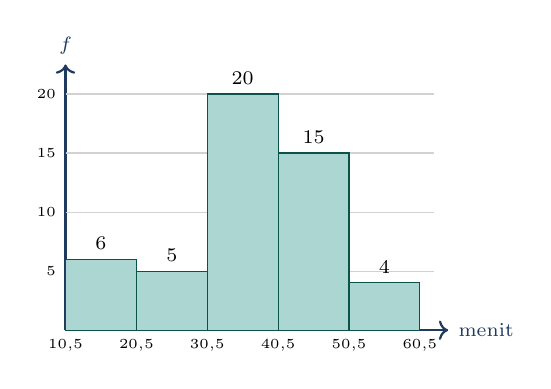
\begin{tikzpicture}[x=0.9cm,y=0.15cm]
\draw[->,thick,navy] (0,0)--(5.4,0) node[right,font=\scriptsize]{menit};
\draw[->,thick,navy] (0,0)--(0,22.5) node[above,font=\scriptsize]{$f$};
\foreach \y in {5,10,15,20}{\draw[gray!35] (0,\y)--(5.2,\y); \node[left,font=\tiny] at (0,\y) {\y};}
\foreach \i/\hh in {1/6,2/5,3/20,4/15,5/4}{
  \fill[teal!35,draw=teal!60!black] (\i-1,0) rectangle (\i,\hh);
  \node[font=\scriptsize,above] at (\i-0.5,\hh) {\hh};}
\foreach \i/\lab in {0/10{,}5,1/20{,}5,2/30{,}5,3/40{,}5,4/50{,}5,5/60{,}5}{\node[font=\tiny,below] at (\i,0) {$\lab$};}
\end{tikzpicture}}}{\poin{8}}

\Needspace{26\baselineskip}
\tingkat{Tingkat Sulit}{soal 3 dan 4}
\soal{Diagram batang berikut menyajikan nilai ulangan matematika siswa kelas A dan kelas B.
\begin{center}
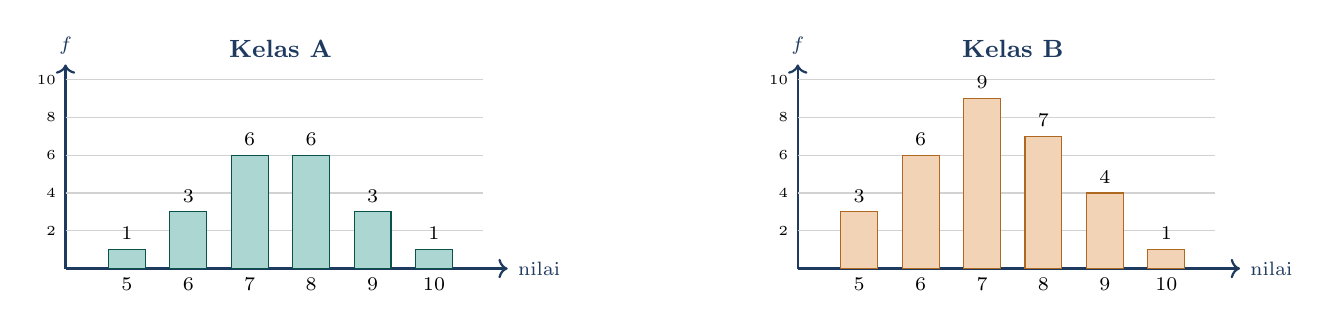
\begin{tikzpicture}[x=0.78cm,y=0.24cm]
\begin{scope}
\node[font=\small\bfseries,navy] at (3.5,11.6) {Kelas A};
\draw[->,thick,navy] (0,0)--(7.2,0) node[right,font=\scriptsize]{nilai};
\draw[->,thick,navy] (0,0)--(0,10.8) node[above,font=\scriptsize]{$f$};
\foreach \y in {2,4,6,8,10}{\draw[gray!35] (0,\y)--(6.8,\y); \node[left,font=\tiny] at (0,\y) {\y};}
\foreach \i/\vv/\fr in {1/5/1,2/6/3,3/7/6,4/8/6,5/9/3,6/10/1}{
  \fill[teal!35,draw=teal!60!black] (\i-0.3,0) rectangle (\i+0.3,\fr);
  \node[font=\scriptsize,above] at (\i,\fr) {\fr};
  \node[font=\scriptsize,below] at (\i,0) {\vv};}
\end{scope}
\begin{scope}[xshift=9.3cm]
\node[font=\small\bfseries,navy] at (3.5,11.6) {Kelas B};
\draw[->,thick,navy] (0,0)--(7.2,0) node[right,font=\scriptsize]{nilai};
\draw[->,thick,navy] (0,0)--(0,10.8) node[above,font=\scriptsize]{$f$};
\foreach \y in {2,4,6,8,10}{\draw[gray!35] (0,\y)--(6.8,\y); \node[left,font=\tiny] at (0,\y) {\y};}
\foreach \i/\vv/\fr in {1/5/3,2/6/6,3/7/9,4/8/7,5/9/4,6/10/1}{
  \fill[amber!35,draw=amber!80!black] (\i-0.3,0) rectangle (\i+0.3,\fr);
  \node[font=\scriptsize,above] at (\i,\fr) {\fr};
  \node[font=\scriptsize,below] at (\i,0) {\vv};}
\end{scope}
\end{tikzpicture}
\end{center}
(a) Tentukan banyak siswa dan rata-rata nilai pada masing-masing kelas.\par
(b) Tentukan median dan modus pada masing-masing kelas.\par
(c) Tentukan rata-rata nilai gabungan seluruh siswa kedua kelas.\par
(d) Siswa dinyatakan tuntas jika nilainya paling sedikit $8$. Hitung persentase siswa yang tuntas pada masing-masing kelas, lalu tentukan kelas mana yang persentase ketuntasannya lebih tinggi.}{\poin{8}}
\soal{Kelas XII-A terdiri atas $24$ siswa dengan rata-rata nilai $70$, sedangkan kelas XII-B terdiri atas $36$ siswa. Rata-rata nilai gabungan kedua kelas adalah $76$.\par\smallskip
(a) Tentukan rata-rata nilai kelas XII-B.\par
(b) Guru menaikkan nilai setiap siswa kelas XII-A sebesar $5$ poin. Tentukan rata-rata nilai gabungan yang baru.\par
(c) Setelah kenaikan pada bagian (b), dua siswa baru dengan nilai yang sama bergabung ke kelas XII-A sehingga rata-rata kelas XII-A menjadi $76$. Tentukan nilai masing-masing siswa baru.\par
(d) Jika rata-rata kelas A tetap $70$ dan rata-rata kelas B tetap seperti hasil (a), tentukan perbandingan banyak siswa kelas A dan kelas B agar rata-rata gabungan menjadi $77$.}{\poin{8}}

\tingkat{Tingkat HOTS}{soal 5}
\soal{Gaji sepuluh pegawai sebuah toko (dalam juta rupiah per bulan) adalah $4,4,5,5,5,6,7,8,9,47$.\par\smallskip
(a) Tentukan rata-rata, median, dan modus gaji tersebut.\par
(b) Pemilik toko mengiklankan bahwa ``gaji rata-rata pegawai kami adalah $10$ juta rupiah per bulan''. Apakah angka itu mewakili gaji pegawai pada umumnya? Ukuran pemusatan mana yang lebih tepat? Jelaskan.\par
(c) Mulai bulan depan gaji setiap pegawai naik $10\%$ dan ditambah tunjangan tetap $0{,}5$ juta, yaitu $y=1{,}1x+0{,}5$. Buktikan bahwa jika $y_i=ax_i+b$ maka $\bar{y}=a\bar{x}+b$, lalu tentukan rata-rata, median, dan modus gaji yang baru.\par
(d) Sebelum kenaikan gaji, toko menerima dua pegawai baru dengan gaji yang sama. Jika rata-rata gaji seluruh $12$ pegawai menjadi $9$ juta, tentukan gaji masing-masing pegawai baru.}{\poin{8}}

% =====================================================================
\newpage
\bagian{Kunci Jawaban dan Pembahasan Singkat}{Untuk guru dan pembahasan mandiri}
\par\vspace{0.6em}{\bfseries\color{navy}Kunci Pilihan Ganda}\par\vspace{0.3em}
\small
\begin{tabularx}{\linewidth}{@{}*{10}{>{\centering\arraybackslash}X}@{}}\hline \textbf{1} & \textbf{2} & \textbf{3} & \textbf{4} & \textbf{5} & \textbf{6} & \textbf{7} & \textbf{8} & \textbf{9} & \textbf{10}\\ \hline B & C & D & A & E & D & C & B & E & A\\ \hline\end{tabularx}\\[6pt]
\begin{tabularx}{\linewidth}{@{}*{10}{>{\centering\arraybackslash}X}@{}}\hline \textbf{11} & \textbf{12} & \textbf{13} & \textbf{14} & \textbf{15} & \textbf{16} & \textbf{17} & \textbf{18} & \textbf{19} & \textbf{20}\\ \hline C & B & D & A & E & B & A & E & D & C\\ \hline\end{tabularx}
\par\vspace{0.8em}{\bfseries\color{navy}\normalsize Pembahasan Pilihan Ganda}\par\vspace{0.2em}
\small\begin{enumerate}[leftmargin=2em,itemsep=2pt,topsep=2pt]
\item[\textbf{1.}] \textbf{(B)} $\bar{x}=\dis\frac{4+6+5+8+7+6+9+5}{8}=\dis\frac{50}{8}=6{,}25$.
\item[\textbf{2.}] \textbf{(C)} Urutkan: $8,9,11,12,14,16,17,21$. Karena $n=8$ (genap), $\Me=\dis\frac{12+14}{2}=13$. (Nilai $13{,}5$ adalah rata-ratanya, bukan median.)
\item[\textbf{3.}] \textbf{(D)} Nilai $5,6,7,8,9$ berfrekuensi $2,5,8,3,2$ sehingga $\sum f=20$ dan $\sum fx=10+30+56+24+18=138$. Maka $\bar{x}=\dis\frac{138}{20}=6{,}9$.
\item[\textbf{4.}] \textbf{(A)} Modus adalah kategori terbanyak, yaitu sektor dengan sudut terbesar (futsal, $108^\circ$). Banyaknya $=\dis\frac{108}{360}\times240=72$ siswa.
\item[\textbf{5.}] \textbf{(E)} Jumlah nilai enam siswa $=6\cdot80=480$ dan jumlah nilai lima siswa $=5\cdot78=390$. Nilai siswa susulan $=480-390=90$.
\item[\textbf{6.}] \textbf{(D)} $\Mo\approx3\,\Me-2\,\bar{x}=3(56)-2(58)=168-116=52$.
\item[\textbf{7.}] \textbf{(C)} Rata-rata dan modus yang baru adalah $1{,}5\bar{x}+4$ dan $1{,}5\Mo+4$. Selisihnya $1{,}5(56-48)=12$. Konstanta $4$ saling meniadakan, tetapi pengali $1{,}5$ ikut mengalikan selisih (jawaban $8$ adalah jebakan karena lupa pengali).
\item[\textbf{8.}] \textbf{(B)} Frekuensi kelas: $4,8,14,10,4$. Kelas modus adalah kelas ketiga dengan $t_b=29{,}5$, $d_1=14-8=6$, $d_2=14-10=4$, $p=5$. Maka $\Mo=29{,}5+\dis\frac{6}{6+4}\cdot5=32{,}5$.
\item[\textbf{9.}] \textbf{(E)} $n=40$, $\dis\frac n2=20$. Kumulatif $6,15,25$, sehingga kelas median $55$--$59$ dengan $t_b=54{,}5$, $F_s=15$, $f=10$, $p=5$. Maka $\Me=54{,}5+\dis\frac{20-15}{10}\cdot5=57$.
\item[\textbf{10.}] \textbf{(A)} Data diukur sampai $0{,}1$ sehingga setengah satuan ukur $=0{,}05$. $t_b=14{,}5-0{,}05=14{,}45$ dan $t_a=16{,}4+0{,}05=16{,}45$. Panjang kelas $p=16{,}45-14{,}45=2{,}0$ (bukan $16{,}4-14{,}5=1{,}9$).
\item[\textbf{11.}] \textbf{(C)} Nilai $84$ tertulis $48$ sehingga jumlah kurang $36$. Nilai $70$ tertulis $79$ sehingga jumlah lebih $9$. Jumlah yang benar bertambah $36-9=27$. Maka $\bar{x}=65+\dis\frac{27}{30}=65{,}9$.
\item[\textbf{12.}] \textbf{(B)} Frekuensi tiap kelas (selisih kumulatif): $6,10,18,10,6$ dengan $n=50$. $\dis\frac n2=25$ dicapai pada kelas $39{,}5$--$49{,}5$ ($F_s=16$, $f=18$, $p=10$): $\Me=39{,}5+\dis\frac{25-16}{18}\cdot10=44{,}5$.
\item[\textbf{13.}] \textbf{(D)} Titik tengah $14{,}5;24{,}5;34{,}5;44{,}5;54{,}5$ berfrekuensi $4,10,16,14,6$ ($n=50$). Pilih $x_s=34{,}5$: $\sum fd=-80-100+0+140+120=80$. Maka $\bar{x}=34{,}5+\dis\frac{80}{50}=36{,}1$.
\item[\textbf{14.}] \textbf{(A)} $\sum x=70$, $n=10$: $\bar{x}=7$; $\Me=\dis\frac{6+6}{2}=6$; $\Mo=6$. (1) benar karena $7>6$. (2) benar: median tetap $6$, rata-rata menjadi $9{,}6$. (3) benar: $\Mo=\Me=6$. (4) salah: setelah dikali $2$, $\bar{x}=14$ dan $\Me=12$, selisihnya $2$.
\item[\textbf{15.}] \textbf{(E)} Misalkan banyak laki-laki $n_L$ dan perempuan $n_P$. $68n_L+75n_P=72(n_L+n_P)\Rightarrow3n_P=4n_L\Rightarrow n_P:n_L=4:3$. (Cara cepat: perbandingan bobot berbanding terbalik dengan jarak ke rata-rata gabungan.)
\item[\textbf{16.}] \textbf{(B)} Urutkan $a\le b\le c\le d\le e$ dengan jumlah $40$ dan $c=9$. Modus tunggal $10$ berarti $10$ muncul paling sedikit dua kali, dan karena $10>9$ maka $d=e=10$. Jadi $a+b=40-9-20=11$. Jika $b=9$, angka $9$ muncul dua kali sehingga modus tidak tunggal; jadi $b\le8$ dan $a\ge3$. Data $3,8,9,10,10$ memenuhi, sehingga nilai terkecil adalah $3$ (jebakan: $2,9,9,10,10$ bermodus ganda).
\item[\textbf{17.}] \textbf{(A)} $6+p+14+q+4=40\Rightarrow p+q=16$. Median $44{,}5$ berada di kelas $40$--$49$ ($t_b=39{,}5$, $F_s=6+p$, $f=14$): $39{,}5+\dis\frac{20-(6+p)}{14}\cdot10=44{,}5\Rightarrow\dis\frac{14-p}{14}=\dis\frac12\Rightarrow p=7$, sehingga $q=9$. Dengan $x_s=44{,}5$: $\sum fd=-120-70+0+90+80=-20$, maka $\bar{x}=44{,}5+\dis\frac{-20}{40}=44$.
\item[\textbf{18.}] \textbf{(E)} Jumlah $=26+x$, rata-rata $=\dis\frac{26+x}{5}$. Tinjau letak $x$: (i) $x\le6$: median $6$, sehingga $\dis\frac{26+x}{5}=6\Rightarrow x=4$ (memenuhi). (ii) $6<x<7$: median $x$, sehingga $26+x=5x\Rightarrow x=6{,}5$ (memenuhi). (iii) $x\ge7$: median $7$, sehingga $\dis\frac{26+x}{5}=7\Rightarrow x=9$ (memenuhi). Jumlah $=4+6{,}5+9=19{,}5$.
\item[\textbf{19.}] \textbf{(D)} Frekuensi $2,5,9,16,8$ ($n=40$). Modus: kelas $70$--$79$, $d_1=7$, $d_2=8$: $\Mo=69{,}5+\dis{\frac{7}{15}}\cdot10\approx74{,}2$. Median: $F_s=16$, $f=16$: $\Me=69{,}5+\dis\frac{20-16}{16}\cdot10=72$. Rata-rata: $\sum fx=89+272{,}5+580{,}5+1192+676=2810$, sehingga $\bar{x}=70{,}25$. Jadi $\bar{x}<\Me<\Mo$ (sebaran condong ke kiri: ekor panjang di kiri menarik rata-rata ke bawah).
\item[\textbf{20.}] \textbf{(C)} Rata-rata gabungan adalah rata-rata berbobot dari $70$ dan $80$, sehingga selalu berada di antara keduanya. Pernyataan (1) saja tidak cukup (tergantung perbandingan banyak siswa). Pernyataan (2) saja tidak cukup (tidak ada informasi rata-rata). Bersama-sama: bobot perempuan lebih dari $\dis\frac12$, sehingga rata-rata gabungan lebih dari $\dis\frac{70+80}{2}=75>74$. Jawabannya pasti ``ya'', jadi keduanya bersama-sama cukup.
\end{enumerate}
\par\Needspace{6\baselineskip}\vspace{0.6em}{\bfseries\color{navy}\normalsize Pembahasan Isian Singkat}\par\vspace{0.2em}
\small\begin{enumerate}[leftmargin=2em,itemsep=2pt,topsep=2pt]
\item[\textbf{1.}] \textbf{Jawaban: $7{,}25$.} $\sum f=20$ dan $\sum fx=10+18+49+40+18+10=145$, sehingga $\bar{x}=\dis\frac{145}{20}=7{,}25$.
\item[\textbf{2.}] \textbf{Jawaban: $162{,}25$ cm.} Titik tengah $152,157,162,167,172$. Dengan $x_s=162$: $d=-10,-5,0,5,10$ dan $\sum fd=-40-40+0+50+40=10$. Maka $\bar{x}=162+\dis\frac{10}{40}=162{,}25$.
\item[\textbf{3.}] \textbf{Jawaban: $51{,}5$.} Frekuensi tiap kelas (selisih berurutan): $6,12,10,8,4$ untuk kelas $29{,}5$--$39{,}5$ sampai $69{,}5$--$79{,}5$. Kumulatif ``kurang dari'': $6,18,28,\dots$; $\dis\frac n2=20$ dicapai di kelas $49{,}5$--$59{,}5$ ($F_s=18$, $f=10$, $p=10$): $\Me=49{,}5+\dis\frac{20-18}{10}\cdot10=51{,}5$.
\item[\textbf{4.}] \textbf{Jawaban: $10$.} $n=25+x$ dan kelas median adalah $21$--$30$ ($t_b=20{,}5$, $F_s=13$, $p=10$). $\Me=20{,}5+\dis\frac{\frac{25+x}{2}-13}{x}\cdot10=25\Rightarrow\dis\frac{5(x-1)}{x}=4{,}5\Rightarrow x=10$. (Cek: $n=35$, $\frac n2=17{,}5$ memang berada di kelas $21$--$30$.)
\item[\textbf{5.}] \textbf{Jawaban: $74$.} Jumlah seluruh $=40\cdot72=2880$. Seperempat terbawah ($10$ siswa): $10\cdot50=500$. Seperempat teratas ($10$ siswa): $10\cdot90=900$. Jumlah $20$ siswa tengah $=2880-500-900=1480$, sehingga rata-ratanya $\dis\frac{1480}{20}=74$.
\end{enumerate}
\par\Needspace{8\baselineskip}\vspace{0.6em}{\bfseries\color{navy}\normalsize Pembahasan dan Pedoman Penskoran Uraian}\par\vspace{0.2em}
\small\begin{enumerate}[leftmargin=2em,itemsep=3pt,topsep=2pt]
\item[\textbf{1.}] (a) Frekuensi nilai $5,6,7,8,9,10$ berturut-turut $2,3,6,5,3,1$ (jumlah $20$). (b) $\sum fx=10+18+42+40+27+10=147$, sehingga $\bar{x}=\dis\frac{147}{20}=7{,}35$. (c) Kumulatif $2,5,11,16,19,20$. Data ke-$10$ dan ke-$11$ sama-sama $7$, sehingga $\Me=\dis\frac{7+7}{2}=7$. Frekuensi terbesar $6$ pada nilai $7$, sehingga $\Mo=7$. (d) Nilai di atas $7{,}35$ adalah $8,9,10$: $5+3+1=9$ siswa, sehingga persentasenya $\dis\frac{9}{20}\times100\%=45\%$. \\ \textit{Penskoran: (a) 2 poin; (b) 2 poin; (c) 2 poin (median 1, modus 1); (d) 2 poin.}
\item[\textbf{2.}] (a) Banyak peserta $=6+5+20+15+4=50$. ``Paling lama $40$ menit'' berarti kelas $11$--$20$, $21$--$30$, dan $31$--$40$ (tepi atas $40{,}5$): $6+5+20=31$ peserta, sehingga persentasenya $\dis\frac{31}{50}\times100\%=62\%$. (b) Titik tengah $15{,}5;25{,}5;35{,}5;45{,}5;55{,}5$. Dengan $x_s=35{,}5$: $\sum fd=-120-50+0+150+80=60$, sehingga $\bar{x}=35{,}5+\dis\frac{60}{50}=36{,}7$ menit. (c) $\dis\frac n2=25$; kumulatif $6,11,31$, sehingga kelas median $31$--$40$ ($t_b=30{,}5$, $F_s=11$, $f=20$): $\Me=30{,}5+\dis\frac{25-11}{20}\cdot10=37{,}5$ menit. (d) Kelas modus $31$--$40$: $d_1=20-5=15$, $d_2=20-15=5$: $\Mo=30{,}5+\dis\frac{15}{20}\cdot10=38$ menit. \\ \textit{Penskoran: (a) 2 poin (banyak peserta 1, persentase 1); (b) 2 poin; (c) 2 poin; (d) 2 poin.}
\item[\textbf{3.}] (a) Kelas A: $n=1+3+6+6+3+1=20$, $\sum fx=5+18+42+48+27+10=150$, $\bar{x}_A=7{,}5$. Kelas B: $n=3+6+9+7+4+1=30$, $\sum fx=15+36+63+56+36+10=216$, $\bar{x}_B=7{,}2$. (b) Kelas A: kumulatif $1,4,10,16,\dots$, data ke-$10$ bernilai $7$ dan ke-$11$ bernilai $8$, sehingga $\Me=7{,}5$; modus $7$ dan $8$ (bimodal). Kelas B: kumulatif $3,9,18,\dots$, data ke-$15$ dan ke-$16$ sama-sama $7$, sehingga $\Me=7$ dan $\Mo=7$. (c) $\bar{x}_{\text{gab}}=\dis\frac{150+216}{20+30}=\dis\frac{366}{50}=7{,}32$ (bukan $\frac{7{,}5+7{,}2}{2}$ karena banyak siswa berbeda). (d) Kelas A: $6+3+1=10$ siswa, $\dis\frac{10}{20}=50\%$. Kelas B: $7+4+1=12$ siswa, $\dis\frac{12}{30}=40\%$. Ketuntasan kelas A lebih tinggi. \\ \textit{Penskoran: (a) 2 poin; (b) 2 poin; (c) 2 poin; (d) 2 poin.}
\item[\textbf{4.}] (a) $24\cdot70+36\,\bar{x}_B=60\cdot76\Rightarrow1680+36\,\bar{x}_B=4560\Rightarrow\bar{x}_B=80$. (b) Rata-rata kelas A menjadi $75$, sehingga $\bar{x}_{\text{gab}}=\dis\frac{24\cdot75+36\cdot80}{60}=\dis\frac{1800+2880}{60}=78$. (c) Jumlah nilai kelas A sekarang $24\cdot75=1800$. Misalkan nilai siswa baru $v$: $\dis\frac{1800+2v}{26}=76\Rightarrow1800+2v=1976\Rightarrow v=88$. (d) $70n_A+80n_B=77(n_A+n_B)\Rightarrow3n_B=7n_A$, sehingga $n_A:n_B=3:7$. \\ \textit{Penskoran: (a) 2 poin; (b) 2 poin; (c) 2 poin; (d) 2 poin.}
\item[\textbf{5.}] (a) $\sum x=100$, sehingga $\bar{x}=10$ juta. Data terurut sudah benar ($n=10$): $\Me=\dis\frac{5+6}{2}=5{,}5$ juta. Modus $=5$ juta (muncul tiga kali). (b) Rata-rata $10$ juta \textbf{tidak mewakili}: sembilan dari sepuluh pegawai bergaji di bawah $10$ juta karena rata-rata terseret pencilan $47$ juta. Median ($5{,}5$ juta) lebih tepat menggambarkan gaji pegawai pada umumnya karena tidak terpengaruh pencilan; modus ($5$ juta) juga menunjukkan gaji yang paling umum. (c) Bukti: $\sum y_i=\sum(ax_i+b)=a\sum x_i+nb$, sehingga $\bar{y}=\dis\frac{a\sum x_i+nb}{n}=a\bar{x}+b$. Dengan $a=1{,}1$ dan $b=0{,}5$: rata-rata baru $=1{,}1(10)+0{,}5=11{,}5$ juta; median baru $=1{,}1(5{,}5)+0{,}5=6{,}55$ juta; modus baru $=1{,}1(5)+0{,}5=6$ juta. (d) Jumlah $12$ pegawai $=12\cdot9=108$ juta, sehingga jumlah dua pegawai baru $=108-100=8$ juta dan gaji masing-masing $4$ juta. \\ \textit{Penskoran: (a) 2 poin; (b) 2 poin (kesimpulan 1, alasan pencilan 1); (c) 2 poin (bukti 1, tiga nilai baru 1); (d) 2 poin.}
\end{enumerate}
\end{document}
